\documentclass{article}
\usepackage[utf8x]{inputenc}
\usepackage[english,russian]{babel}
\usepackage{geometry}
  \geometry{left=2cm}
  \geometry{right=1.5cm}
  \geometry{top=1cm}
  \geometry{bottom=2cm}
\usepackage{tikz}
\usepackage{multicol}
\usepackage{listings}

\begin{document}
\pagestyle{plain}
\lstset{
  language=C,                % choose the language of the code
  basicstyle=\linespread{1.1}\ttfamily,
  columns=fixed,
  fontadjust=true,
  basewidth=0.5em,
  keywordstyle=\color{blue}\bfseries,
  commentstyle=\color{gray},
  stringstyle=\ttfamily\color{orange!50!black},
  showstringspaces=false,
  numbersep=5pt,
  numberstyle=\tiny\color{black},
  numberfirstline=true,
  stepnumber=1,                   % the step between two line-numbers.        
  numbersep=10pt,                  % how far the line-numbers are from the code
  backgroundcolor=\color{white},  % choose the background color. You must add \usepackage{color}
  showstringspaces=false,         % underline spaces within strings
  captionpos=b,                   % sets the caption-position to bottom
  breaklines=true,                % sets automatic line breaking
  breakatwhitespace=true,         % sets if automatic breaks should only happen at whitespace
  xleftmargin=.2in,
  extendedchars=\true,
  keepspaces = true,
}
\lstset{literate=%
   *{0}{{{\color{red!20!violet}0}}}1
    {1}{{{\color{red!20!violet}1}}}1
    {2}{{{\color{red!20!violet}2}}}1
    {3}{{{\color{red!20!violet}3}}}1
    {4}{{{\color{red!20!violet}4}}}1
    {5}{{{\color{red!20!violet}5}}}1
    {6}{{{\color{red!20!violet}6}}}1
    {7}{{{\color{red!20!violet}7}}}1
    {8}{{{\color{red!20!violet}8}}}1
    {9}{{{\color{red!20!violet}9}}}1
}

\title{Семинар \#4: Часть 2: Структуры. Классные задачи.\vspace{-5ex}}\date{}\maketitle

\section*{Основы структур}

Структуры -- это композитный тип данных, объединяющий набор объектов в один объект. Используя структуры, мы можем сами создать новый тип данных, используя другие типы как кирпичики.
Предположим, что мы разрабатываем приложение для работы с двумерной графикой и нам понадобилось как-то описывать точку в двумерном пространстве. Для этого  мы можем опеределить структуру точки, как это сделано в следующем примере:
\begin{lstlisting}
#include <stdio.h>

struct point 
{
    float x;
    float y;
};

int main() 
{
    struct point a = {0.0, 1.1};
    a.x = 2.2;
    printf("(%g, %g)\n", a.x, a.y); // Напечатает (2.2, 1.1)
}
\end{lstlisting}
\subsubsection*{Пояснение по коду:}
\begin{itemize}
\item Сначала мы определили новую структуру с двумя полями \texttt{x} и \texttt{y} типа \texttt{float}. После того, как мы это сделали у нас появился новый тип данных по имени \texttt{struct point} (да, название типа состоит из двух слов).
\item \texttt{!} Не забывайте ставить точку с запятой в конце определения структуры. Это нужно делать обязательно. 
\item Далее, в функции \texttt{main}, создаём переменную типа \texttt{struct point} по имени \texttt{a} и сразу инициализируем её.
\item Переменная \texttt{a} типа \texttt{struct point} хранит в себе два объекта типа \texttt{float} по имени \texttt{x} и \texttt{y}.
\item Получить доступ к внутренностям переменной \texttt{a} можно с помощью оператора \texttt{.} (точка).
\end{itemize}



\subsection*{Допустимые операции со структурами}
\begin{enumerate}
\item При создании структуры её элементы можно инициализировать с помощью фигурных скобочек.
\begin{lstlisting}
struct point a = {2.1, 4.3};
\end{lstlisting}
Однако нельзя таким образом присваивать
\begin{lstlisting}
a = {5.6, 7.8}; // Ошибка, фигурными скобочками можно только инициализировать!
\end{lstlisting}
\item Доступ к элементу структуры осуществляется с помощью оператора точка
\begin{lstlisting}
a.x = 5.6;
a.y = 7.8;
\end{lstlisting}
\item Структуры можно присваивать друг другу. При этом происходит побайтовое копирование содержимого одной структуры в другую.
\begin{lstlisting}
struct point b;
b = a;
\end{lstlisting}
\end{enumerate}

\subsection*{Массив структур}
Структуры, как и обычные переменные, можно хранить в массивах. В примере ниже создан массив под названием \texttt{array}, содержащий в себе 3 точки.
\begin{lstlisting}
#include <stdio.h>

struct point 
{
    float x
    float y;
};

int main() 
{
    struct point array[3] = {{1.1, 2.2}, {3.3, 4.4}, {5.5, 6.6}};
    array[1].y = 9.9;
    printf("(%g, %g)\n", array[1].x, array[1].y); // Напечатает (3.3, 9.9)
}
\end{lstlisting}

\subsection*{Передача структуры в функцию}
Структуры можно передавать в функции и возвращать из функций также как и обычные переменных. При передаче в функцию происходит полное копирование структуры и функция работает уже с копией структуры. При возвращении из функции также происходит копирование.
\begin{lstlisting}
#include <stdio.h>

struct point 
{
    float x;
    float y;
};

void print_point(struct point a) 
{
    printf("(%g, %g)", a.x, a.y);
}

struct point add_points(struct point a, struct point b) 
{
    struct point result;
    result.x = a.x + b.x;
    result.y = a.y + b.y;
    return result;
}

int main() 
{
    struct point a = {1.1, 2.2}; 
    struct point b = {3.3, 4.4};
    struct point c = add_points(a, b);
    print_point(c);
}
\end{lstlisting}

\newpage
\subsection*{Структуры содержащие более сложные типы данных}
Структуры могут содержать в себе не только базовые типы данных, но и более сложные типы, такие как массивы (в том числе строки), указатели, а также другие структуры.\\
Пример программы, в которой описывается структура для удобной работы с объектами Книга (\texttt{struct book}).
\begin{lstlisting}
#include <stdio.h>
#include <string.h>

struct book 
{
    char title[50];
    int pages;
    float price;
};

void print_book(struct book b) 
{
    printf("Book info:\n");
    printf("Title: %s\nPages: %d\nPrice: %g\n\n", b.title, b.pages, b.price);
}

int main() 
{
    struct book a = {"The Martian", 10, 550.0};
    print_book(a);
    
    a.pages = 369;
    strcpy(a.title, "The Catcher in the Rye");
    print_book(a);
    
    struct book scifi_books[10] = 
    {
        {"Dune", 300, 500.0}, 
        {"Fahrenheit 451", 400, 700.0},
        {"Day of the Triffids", 304, 450.0}
    };
    scifi_books[2].price = 2000.0;
    print_book(scifi_books[2]);
}
\end{lstlisting}
\newpage
\section*{Указатели на структуры:}
Указатель на структуру хранит адрес первого байта структуры. Для доступа к полям структуры по указателю нужно сначала этот указатель разыменовать, а потом использовать: \texttt{(*p).price}. Для удобства был введён оператор стрелочка \texttt{->}, который делает то же самое: \texttt{p->price}.
\begin{multicols}{2}
\begin{lstlisting}
#include <stdio.h>

struct book 
{
    char title[50];
    int pages;
    float price;
};

int main() 
{
    struct book a = {"The Martian",277,540};
    struct book* p = &a;
    
    // Три способа доступа к полю:
    a.price += 10;
    (*p).price += 10;
    p->price += 10;
}
\end{lstlisting}
\vfill\null
\columnbreak
\vspace*{3\baselineskip}
\begin{center}
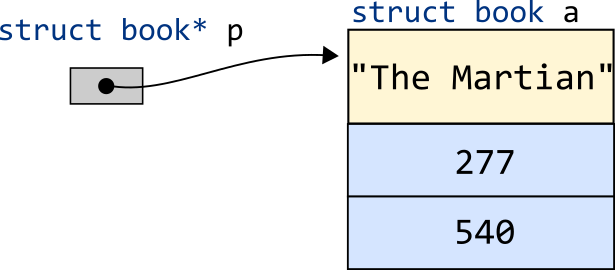
\includegraphics[scale=0.5]{../images/structpointer2.png}
\end{center}
\end{multicols}


\subsection*{Передача по значению}
При обычной передаче в функцию всё содержимое копируется. Функция работает с копией.
\begin{multicols}{2}
\begin{lstlisting}
#include <stdio.h>

struct book 
{
    char title[50];
    int pages;
    float price;
};
void change(struct book a) 
{
    a.price += 10;
}
int main()
{
    struct book a = {"The Martian",277,540};
    change(a); // внутри функции структура a НЕ изменится
}
\end{lstlisting}
\vfill\null
\columnbreak
\vspace*{3\baselineskip}
\begin{center}
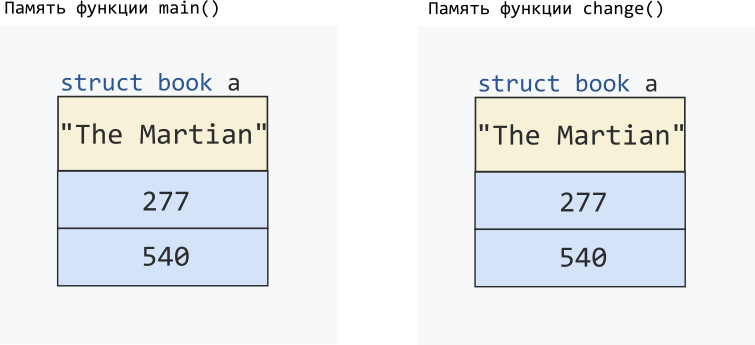
\includegraphics[scale=0.5]{../images/structpassbyvalue.png}
\end{center}
\end{multicols}


\subsection*{Передача по указателю}
При передаче в функцию по указателю копируется только указатель.
\begin{multicols}{2}
\begin{lstlisting}
#include <stdio.h>

struct book 
{
    char title[50];
    int pages;
    float price;
};
void change(struct book* p) 
{
    p->price += 10;
}
int main() 
{
    struct book a = {"The Martian",277,540};
    struct book* p = &a;
    change(p); // внутри функции структура a изменится
}
\end{lstlisting}
\vfill\null
\columnbreak
\begin{center}
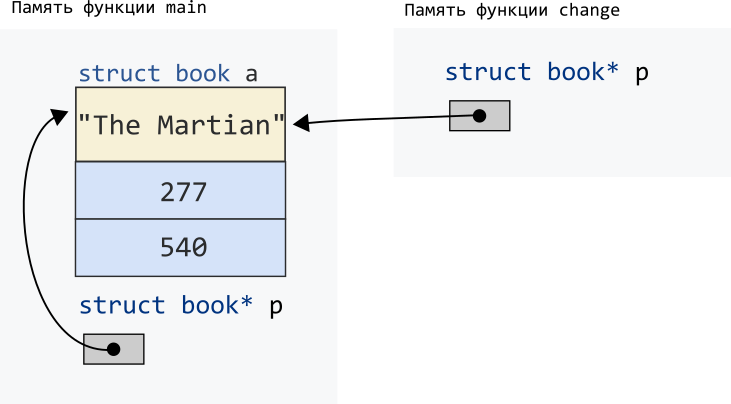
\includegraphics[scale=0.5]{../images/structpassbypointer.png}
\end{center}
\end{multicols}

Такой способ передачи имеет 2 преимущества:
\begin{enumerate}
\item Можно менять структуру внутри функции, и изменения будут действительны вне функции
\item Не приходится копировать структуры, поэтому программа работает быстрее.
\end{enumerate}

\subsection*{Передача по константному указателю}
Иногда мы не хотим менять структуру внутри функции, но хотим чтобы ничего не копировалось. Тогда желательно использовать передачу по константному указателю.
\begin{lstlisting}
#include <stdio.h>

struct book 
{
    char title[50];
    int pages;
    float price;
};

void print_book_info(const struct book* p) 
{
    printf("Title: %s\nPages: %d\nPrice: %g\n\n", p->title, p->pages, p->price);
}

int main() 
{
    struct book a = {"The Martian",277,540};
    print_book_info(&a);
}
\end{lstlisting}
\newpage


\newpage
\section*{Выравнивание}
Пусть есть структура \texttt{struct test} и нам нужно узнать её размер если размеры типов \texttt{char}, \texttt{int} и \texttt{double} равны \texttt{1}, \texttt{4} и \texttt{8} байт соответственно.
\begin{lstlisting}
struct test 
{
    int a;
    char b;
    double c;
};
\end{lstlisting}
Кажется, что размер этой структур равен сумме размеров состовляющих её элементов, то есть \texttt{13}. Но это не так. 
На самом деле размер этой структуры будет отличаться в зависимости от вычислительной системы, на которой запускается код (как, впрочем, и размеры других типов). Но на большинстве вычислительных систем размер структуры \texttt{struct test} будет больше суммы состовляющих её элементов. Это можно проверить с помощью следующего кода:


\begin{lstlisting}
int main() 
{
    printf("Size of char   = %zu\n", sizeof(char));
    printf("Size of int    = %zu\n", sizeof(int));
    printf("Size of double = %zu\n", sizeof(double));
    printf("Size of test   = %zu\n", sizeof(struct test));
}
\end{lstlisting}

Причина по которой это происходит заключается в том, что система значительно быстрей работает с данными, если они лежат в памяти по адресам, кратным 4-м или 8-ми. Поэтому компилятор автоматически выравнивает элементы структуры в памяти так, чтобы их адреса были кратны некоторой степени двойки.

Для того, чтобы найти величину выравнивания можно использовать оператор \texttt{\_Alignof}:
\begin{lstlisting}
#include <stdio.h>

int main() 
{
    int a = 10;
    printf("Alignment of int = %zu\n", _Alignof(int));
    printf("Alignment of int = %zu\n", _Alignof(a));
}
\end{lstlisting}




\end{document}